
%
% # INTRODUCTION:
%
% This write up is for Lab2: Verification of Equivalent Logic Functions
%
% Specifically this was used for the class Logic Design Fundamentals (EECE 144)
% taught by Kurtis Kredo [http://www.ecst.csuchico.edu/~kkredo/]
% during the Fall 2011 semester at CSU Chico [www.csuchico.edu].
% 
% ## LaTeX
%
% This file is written for LaTeX [http://www.latex-project.org/]
% which is used to process this file in to a completely formatted
% document.
%
% If you are unfamiliar with LaTeX it can seem daunting at first
% (as with anything new) but there are many benefits.
% Imagine writing a document in Word except without
% having to worry about the tedious things such as line breaks,
% indentation, table of contents, appendices, font styles,
% heading sizes, citations/references, page numbers.
% LaTeX lets you focus on the content without
% worrying about the tedious details.  It is also excellent for
% producing mathematical formulas.
% 
% If you are collaborating with someone else you can simply edit
% the sections and paragraphs in this file as needed.
%
% To process this file use a command such as 'rubber'.
%
%   bash$ rubber skel.tex
%   (output to skel.dvi)
%   bash% rubber --pdf skel.tex
%   (output to skel.pdf)
%
% # AUTHORS (of this template):
%
%   Jeremiah Mahler <jmmahler@gmail.com>
%   https://www.google.com/profiles/jmmahler#about 
%
% # COPYRIGHT:
%
%   Copyright (C)  2011 Jeremiah Mahler <jmmahler@gmail.com>.
%   Permission is granted to copy, distribute and/or modify this document
%   under the terms of the GNU Free Documentation License, Version 1.3
%   or any later version published by the Free Software Foundation;
%   with no Invariant Sections, no Front-Cover Texts, and no Back-Cover Texts.
%   A copy of the license is included in the file "fdl-1.3.txt".
%

\documentclass[12pt]{article}
%\documentclass[10pt]{article}

%\usepackage{mslapa}
\usepackage{hyperref}
\usepackage{amsmath}
\usepackage{graphicx}
\usepackage{ulem}
%\usepackage{vmargin}
\usepackage{tabularx}
\usepackage{sectsty}
\usepackage{pbox}
\usepackage{bigstrut}
\usepackage{enumerate}

%\usepackage{cleveref}

%\setpapersize{USletter}
\sectionfont{\normalsize}
\subsectionfont{\normalsize}

% configure \bigstrut size
% This configures spacing above and below rows in a tabularx.
%\renewcommand{\bigstrutjot}{6pt}
\renewcommand{\bigstrutjot}{2.0\jot}

\setlength{\parindent}{0in}

\begin{document}

% {{{ Cover Page

\centerline{\bf EECE 144}
\centerline{\bf Fall 2011}
\centerline{\bf}
\centerline{\bf Lab Report \#2}
\centerline{\bf Section 4}
\centerline{\bf 9/14/2011}

% signature area
\begin{center}
\begin{tabularx}{\textwidth}[b]{X l l}
Submitted by: & & \\
Signature & Printed Name & Date \\
\hline
\multicolumn{1}{|X|}{} & \multicolumn{1}{|l|}{\bigstrut \bf Jeremiah Mahler} & \multicolumn{1}{|l|}{\bf Sep 14, 2011} \\
\hline
\multicolumn{1}{|X|}{} & \multicolumn{1}{|l|}{\bigstrut \bf Marvanee Johnson} & \multicolumn{1}{|l|}{\bf Sep 14, 2011} \\
\hline
\end{tabularx}
\end{center}
% }}}

\section{Description/Objectives}

This lab illustrates how create and verify equivalent logic functions
manually and with Logisim \cite{LOGISIM}.

\section{Procedure}

Given two different logic functions (Equations \ref{eq:fn1}, \ref{eq:fn2})
the task is to verify that they are logically equivalent.

\begin{align}
& a b + c' + abc \label{eq:fn1} \\
& a b + c' \label{eq:fn2}
\end{align}

For each logic function the following steps are performed:
\begin{enumerate}
	\item Define the function with logic gates in Logisim.
	\item Using the Logisim simulation generate all combinations of
	inputs and record the corresponding output as a truth table.
	\item Manually calculate the outputs for every combination of inputs
	as a second truth table.
	\item Verify that the simulated outputs are the same as the
	manually calculated outputs.
\end{enumerate}

As a final step, since we know the functions are equivalent, we algebraically
manipulate one of the given functions in to the form of the second function.

\subsection{Verify $a b + c' + abc$}
\label{sec:verfirst}

Figure \ref{fig:logisim1} shows the circuit as it was defined in Logisim.
Figure \ref{fig:out1} shows the output from Logisim and the manual calculations.

\begin{figure}[!hbtp]
\center
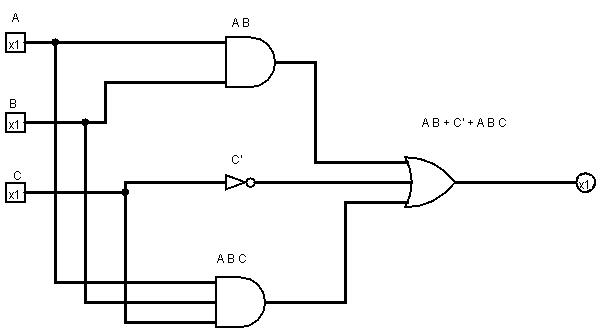
\includegraphics[scale=0.5]{img/Lab2-01}
\caption{Logic circuit $a b + c' + a b c$ defined in Logisim.}
\label{fig:logisim1}
\end{figure}


\begin{figure}[!hbt]

\center

\begin{tabular}[t]{| l | l | l | l | l |}
\hline
\multicolumn{5}{| c |}{$a b + c' + abc$} \\
\hline
$a$ & $b$ & $c$ & Logisim out & manual out \\
\hline
0 & 0 & 0 & 1 & 1 \\
\hline
0 & 0 & 1 & 0 & 0 \\
\hline
0 & 1 & 0 & 1 & 1 \\
\hline
0 & 1 & 1 & 0 & 0 \\
\hline
1 & 0 & 0 & 1 & 1 \\
\hline
1 & 0 & 1 & 0 & 0 \\
\hline
1 & 1 & 0 & 1 & 1 \\
\hline
1 & 1 & 1 & 1 & 1 \\
\hline
\end{tabular}

\caption{Truth table of outputs for the function $a b + c' + a b c$ simulated
in Logisim and calculated manually.}
\label{fig:out1}
\end{figure}


\subsection{Verify $a b + c'$}
\label{sec:versecond}

Figure \ref{fig:logisim2} shows the circuit as it was defined in Logisim.
Figure \ref{fig:out2} shows the output from Logisim and the manual calculations.


\begin{figure}[!hbtp]
\center
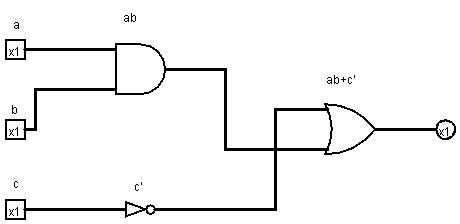
\includegraphics[scale=0.5]{img/Lab2-02}
\caption{Logic circuit $a b + c'$ defined in Logisim.}
\label{fig:logisim2}
\end{figure}


\begin{figure}[!hbt]

\center

\begin{tabular}[t]{| l | l | l | l | l |}
\hline
\multicolumn{5}{| c |}{$a b + c'$} \\
\hline
$a$ & $b$ & $c$ & Logisim out & manual out \\
\hline
0 & 0 & 0 & 1 & 1 \\
\hline
0 & 0 & 1 & 0 & 0 \\
\hline
0 & 1 & 0 & 1 & 1 \\
\hline
0 & 1 & 1 & 0 & 0 \\
\hline
1 & 0 & 0 & 1 & 1 \\
\hline
1 & 0 & 1 & 0 & 0 \\
\hline
1 & 1 & 0 & 1 & 1 \\
\hline
1 & 1 & 1 & 1 & 1 \\
\hline
\end{tabular}

\caption{Truth table of outputs for the function $a b + c'$ simulated
in Logisim and calculated manually.}
\label{fig:out2}
\end{figure}

\subsection{Reduction of $a b + c' + abc$ in to $a b + c'$}
\label{sec:verboth}

Additionally, to verify that the logic functions are equivalent,
the first function ($a b + c' + a b c$) is algebraically manipulated/reduced
using the Laws of Boolean Algebra \cite[Pg. 55]{roth2009fundamentals}
in to the form of the second ($a b + c'$) as shown in Figure \ref{fig:red}.

\begin{figure}
\begin{align*}
a b + c' &+ abc 	&& \\
a b + abc &+ c' 	&& \quad \mbox{(Commutative Law)} \\
a (b + bc) &+ c' 	&& \quad \mbox{(Distributive Law)} \\
a (b (1 + c)) &+ c' && \quad \mbox{(Distributive Law)} \\
a b &+ c' 			&& \quad \mbox{($0/1$ Law, $X + 1 = 1$))}
\end{align*}

\caption{Reduction of $ab + c' + abc$ in to $ab + c'$}
\label{fig:red}
\end{figure}

\section{Observations}

For both functions it was found that the circuit created in Logisim
agreed with the expected behaviour as was calculated manually.
And it was found through reduction using Boolean Algebra that the
both functions were logically equivalent.

%\clearpage

\section{Conclusion}

This lab was a success in showing that there are various ways to
verify logic functions that appear to be different to see if they
are logically equivalent.
The functions can be manually calculated or simulated in Logisim.
And the output for every possible combination can be organized
in a truth table for comparison.
The functions can also be algebraically manipulated using Boolean Algebra
to show if they are equivalent.

% flush all the figures
%\clearpage

%\pagebreak
\renewcommand*{\refname}{\vspace{-8mm}}
\section{References}
%\bibliographystyle{plain}
%\bibliographystyle{mslapa}
\bibliographystyle{ieeetr}
\bibliography{../references}

% Appendix (if needed)

\end{document}

% vim:foldmethod=marker
